\chapter{Системийн зохиомж}
Орчин үеийн үүлийн технологид суурилсан тоон гарын үсгийн систем хийх болсонтойгоор холбоотой хийсэн судалгаанууд.
\section{Тоон гарын үсгийн стандарт}.
Хэдийгээр бүх цахим гарын үсэг нь DSS-ийн дүрмийг дагаж мөрдөх ёстой боловч тэдгээр нь бүгд адилхан биш юм. Баримт бичигт гарын үсэг зурахад ашиглаж болох гурван төрлийн тоон гарын үсгийн стандарт байдаг.
\begin{enumerate}
	\item \textbf{Энгийн цахим гарын үсэг (SES)} - Цахим гарын үсгийн хамгийн үндсэн хэлбэр. SES нь баримт бичигт нэмэхэд хурдан бөгөөд хялбар боловч шифрлэлтийн аргаар хамгаалагдаагүй. Өөрөөр хэлбэл, тийм ч аюулгүй биш юм. Үүнд жишээ нь цахим шуудангийн гарын үсэг ордог.
	\item \textbf{Нарийвчилсан цахим гарын үсэг (AES)} - Хэдийгээр хууль ёсны дагуу хүчингүй боловч AES (Advanced Electronic Signature) нь гарын үсэг зурсны дараа баримт бичигт өөрлчлөлт орсон эсэхийг мэдэх боломжтой крифтографыг ашигладаг. Гэсэн хэдий ч хуулийн дагуу хүчингүй хэвээр.
	\item \textbf{Qualified advanced electronic signature (QES)} - Цахим хэлбэрээр гарын үсэг зурах хамгийн найдвартай арга. Тоон гарын үсэг гэж нэрлэгддэг шаардлага хангасан цахим гарын үсэг нь аюулгүй байдлын дээд түвшинг хангахын тулд нийтийн түлхүүрийн дэд бүтэц, тэгш бус криптограф, Two Factor баталгаажуулалтыг ашигладаг. Эдгээрийг ашигласнаар, гарын үсэг нь хууль ёсны дагуу хүчийн төгөлдөр болно.
\end{enumerate}
\section{Адил системийн судалгаа}
\subsubsection{Tridumkey.mn}
Tridimkey нь Монгол улсын бүртгэлийн ерөнхий газраар хүлээн зөвшөөрөгдсөн тоон гарын үсэг олгогч ба байгуулагад зориулж гарын үсэг олгодог нь онцлог санагдсан. Байгууллагад зориулж гарын үсэг авахад бүрдүүлдэг баримтууд.
\begin{enumerate} 
	\item Иргэний үнэмлэх эх хувь эсвэл И-монголиа-ийн иргэний  үнэмлэхийн лавлагаа		
	\item Байгууллагын гэрчилгээ		
	\item Албан бичиг эх хувь		Загвар татах
	\item Эзэмшигч өөрийн биеээр ирэх боломжгүй үед итгэмжлэлтэй албан бичиг
	\item Анкет
\end{enumerate}
Гэвч сул тал нь энэхүү тоон гарын үсгийн систем нь зөвхөн \textbf{Windows} үйлдлийн систем дээр ажилдаг ба Macos эсвэл Linux үйлдлийн систем ашигладаг хэрэглэгчид ашиглах боломжгүй болж байгаа юм.
\subsubsection{Monpass.mn}
"Таньж баталгаажуулах тоон гарын үсгийн гэрчилгээ: Цахим бизнес, төрийн болон бусад төрөл бүрийн систем, онлайн үйлчилгээнд хандах, бусад цахим гүйлгээ, хэлцэл хийхэд найдвартай таньж баталгаажуулах, захидал харилцааг хөдөлбөргүй баталгаажуулахын тулд тоон гарын үсэг зурах, захидал харилцаа, дамжуулж буй баримт бичгийг шифрлэн дамжуулах, ажилтнууд, хэрэглэгчдийг хялбар таних, бөөний онлайн худалдаа зохион байгуулах гэх мэт зорилгоор ашиглагддаг тоон гарын үсгийн гэрчилгээ – цахим баримт бичиг юм. Энэ гэрчилгээ нь хэрэглэгчийн мэдээлэл, олгосон ГОБ-ын мэдээлэл, хосгүй серийн дугаар болон бусад хосгүй өгөгдлүүд, хүчинтэй хугацаа, тоон гарын үсгийн нийтийн түлхүүр, холбогдох бусад мэдээллийг агуулсан байх бөгөөд Хувь хүмүүс болон байгууллагын төлөөлөгч хэн боловч ашиглаж болно. Захидал, мэдээлэлдээ тоон гарын үсэг зурахдаа өөрийн тоон гарын үсгийн хувийн түлхүүрийг ашиглах ба харин шифрлэн илгээх бол хүлээн авагчийн нийтийн түлхүүрийг ашиглана." гэсэн танилцуулагатай байсан ба гүнзгий судалж үзэхэд мөн л хэрэглэгчийн үйлдлийн систем зөвхөн \textbf{Windows} байж л тоон гарын үсгийн ашиглах боломжтой байсан юм.
\pagebreak
\section{Системийн шаардлага}
\subsubsection{Функциональ шаардлага}
% table
\begin{table}[h]
	\centering
	\caption{Функциональ шаардлага}
	\begin{tabular}{ |p{2cm}|p{13cm}| }
	\hline
	ФШ 100 &  Систем нь хэрэглэгчийн тоон гарын үсэг үүсгэх чадвартай байх ёстой. Үүнд хэрэглэгч бүрийн өвөрмөц түлхүүрийн хослолыг бий болгох орно. \\ \hline
	ФШ 200 &  Систем нь тоон гарын үсгийг баталгаажуулах функцээр хангах ёстой. Энэ нь гарын үсэг зурсан баримт бичгийг хүлээн авч, гарын үсэг зурсан хүний нийтийн түлхүүрийг ашиглан гарын үсгийг баталгаажуулах ёстой. \\ \hline
	ФШ 300 &  Систем нь хэрэглэгчдэд гарын үсэг зурахын тулд янз бүрийн форматтай цахим баримт бичгүүдийг (жишээлбэл, .doc, .pdf, .xls гэх мэт) байршуулахыг зөвшөөрөх ёстой. \\ \hline
	ФШ 400 &  Систем нь хэрэглэгчдийг баримт бичигт гарын үсэг зурах, баталгаажуулахаас өмнө баталгаажуулах ёстой. Үүнийг хэрэглэгчийн нэр/нууц үг, олон хүчин зүйлийн баталгаажуулалт эсвэл бусад аюулгүй аргуудаар хийж болно. \\ \hline
	ФШ 500 &  Систем нь баримт бичиг байршуулах, гарын үсэг үүсгэх, гарын үсгийн баталгаажуулалт зэрэг хэрэглэгчдийн хийсэн бүх үйлдлийг бүртгэх ёстой. \\ \hline
	ФШ 600 &  Систем нь бусад үйлчилгээтэй нэгтгэх API-г өгөх ёстой. Энэ нь бусад програм хангамж эсвэл үйлчилгээнд энэ үйлчилгээний тоон гарын үсгийн чадварыг ашиглах боломжийг олгоно. \\  \hline
	ФШ 700 &  Веб нь хэрэглэгч бүртгэх боломжтой байх \\ \hline
\end{tabular}
\end{table}
\subsubsection{Функциональ бус шаардлага}
% table
\begin{table}
	\centering
	\caption{Функциональ бус шаардлага}
	\begin{tabular}{ |p{2cm}|p{13cm}| }
	\hline
	ФБШ 100 &  Систем нь GDPR эсвэл HIPAA гэх мэт холбогдох бүх мэдээллийн аюулгүй байдал, нууцлалын дүрэм журмыг дагаж мөрдөх ёстой. Гарын үсэг, баримт бичиг зэрэг бүх өгөгдөл шифрлэгдсэн байх ёстой. \\ \hline
	ФБШ 200 &  Систем нь гүйцэтгэлийн бууралтгүйгээр олон тооны хэрэглэгчид болон баримт бичгүүдийг зохицуулах чадвартай байх ёстой. \\ \hline
	ФБШ 300 &  Үүлэн үйлчилгээ нь хамгийн бага зогсолттой, 24/7 цагийн турш ашиглах боломжтой байх ёстой. Үйлчилгээний түвшний гэрээ (SLA) нь дор хаяж 99.9\% ажиллах хугацааг баталгаажуулах ёстой. \\ \hline
	ФБШ 400 &  Систем нь хүлээн зөвшөөрөгдсөн тодорхой хугацааны дотор гарын үсэг үүсгэх, баталгаажуулах хүсэлтийг хурдан боловсруулах чадвартай байх ёстой. \\ \hline
	ФБШ 500 &  Систем нь янз бүрийн техникийн чадвартай хэрэглэгчдэд үүнийг үр дүнтэй ашиглах боломжийг олгодог хэрэглэгчдэд ээлтэй интерфэйстэй байх ёстой. \\ \hline
	ФБШ 600 &  Үүлэн үйлчилгээ нь янз бүрийн үйлдлийн систем, хөтөч, төхөөрөмжтэй нийцтэй байх ёстой. \\  \hline
	ФБШ 700 &  Энэ систем нь гамшгийн үед өгөгдөл алдагдахгүй байхын тулд найдвартай нөөцлөх, сэргээх механизмтай байх ёстой. \\ \hline
	ФБШ 800 &  Систем нь Европ дахь eIDAS эсвэл АНУ-ын ESIGN хууль зэрэг тоон гарын үсгийн хууль тогтоомж, дүрэм журамд нийцсэн байх ёстой.\\ \hline
\end{tabular}
\end{table}
\newpage
\section{Use case диаграм}
\begin{figure}[h]
	\centering
	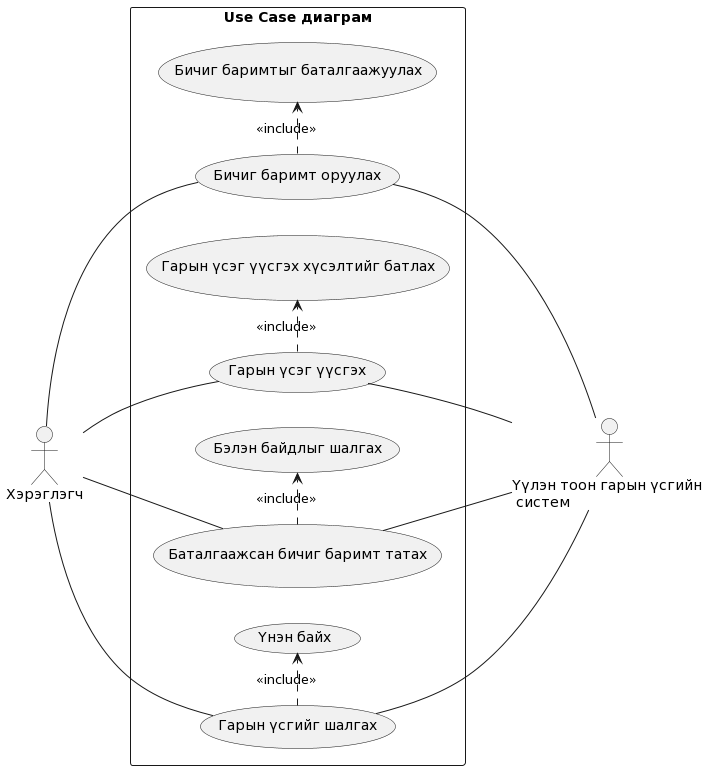
\includegraphics[scale=0.56]{assets/usecase_mn.png}
	\caption{Use case диаграм}
	\label{fig:usecasemn}
\end{figure}
\section{ER диаграм}
\begin{figure}
	\centering
	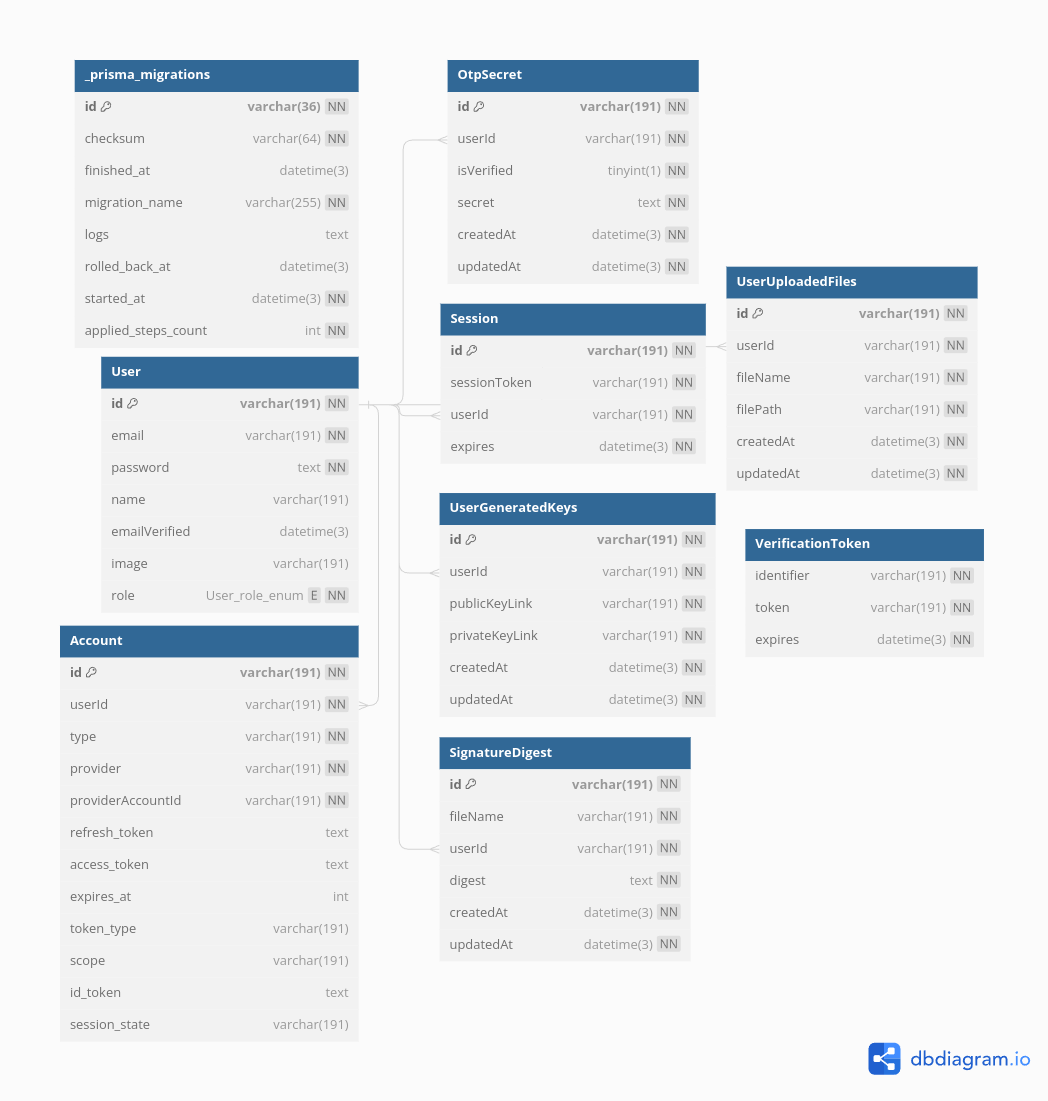
\includegraphics[scale=0.43]{assets/cryptography.png}
	\caption{Датабаз диаграм}
	\label{fig:dbdiagram}
\end{figure}